%!TEX root = ../../Main.tex
\graphicspath{{Chapters/Design/}}
%-------------------------------------------------------------------------------

\chapter{Design}
\label{cha:design}

The principals of SAMVIQ should be incorporated in a software application which the observer can use to evaluate images. The first choice to make is whether the application should be PC or web based. PC applications are confined to a physical location and hence have usability constraints. Web applications on the other hand make it convenient for the observer to access the application from any location using the Internet. Due to the exact evaluation scenario is unknown it is chosen to make the application web based in order to enhance flexibility.

The programming language used for the application is specified by the supervisor of this project to be Python. To ease the development process it is chosen to base the development on a web application framework. The chosen framework is Django \cite{django} which is the largest Python-based web framework. Online remarks of the Django framework includes; "Django aims to include all the batteries a web application will need so developers need only open the box and start working, pulling in Django's many modules as they go." \cite{airpair} and "Django is great for developers who want to build something quickly with powerful built-in tools"\cite{six_feet_up}. Alternatives to Django would be Flask\cite{flask} and Pyramid\cite{pyramid}.

\section{The web application} % (fold)
\label{sec:the_web_application}

The framework architecture is inspired by the Model View Controller (MVC) architecture and consists of four instances; a model, a view, a template, and an URL dispatcher. The model describes the data in the database. The template defines how observers see things in the browser. The view controls what observers see and the communication between the template and the model. The URL dispatcher maps the requested URL to a view function and calls it. The architecture is illustrated in \autoref{fig:django_architecture}.

\begin{figure}[H]
	\centering
	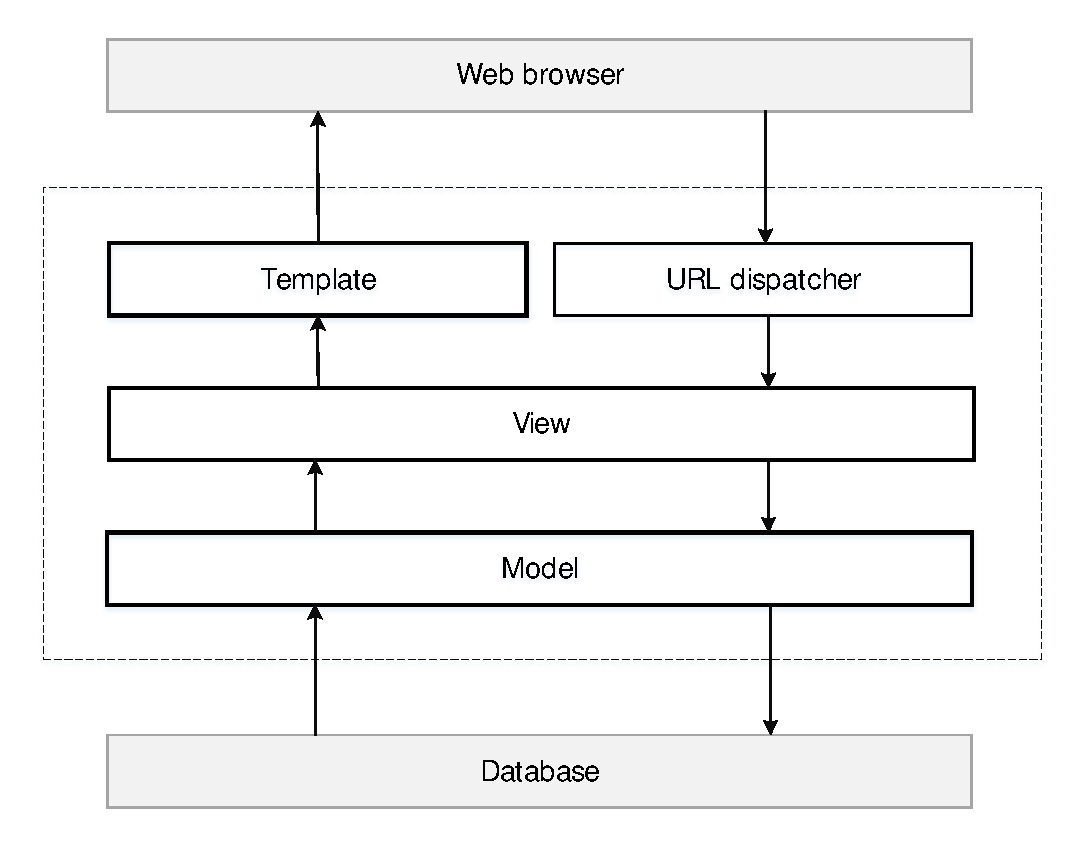
\includegraphics[width = 250pt]{Img/Architecture.pdf}
	\caption{The architecture of the Django framework.}
	\label{fig:django_architecture}
\end{figure}

\subsection{Model} % (fold)
\label{sub:model}

The model defines the data and the interaction with the database. The database is a SQLite database which consists of three tables; Observer, Image, and Rating. This is illustrated in \autoref{fig:database_architecture}.

\begin{figure}[H]
	\centering
	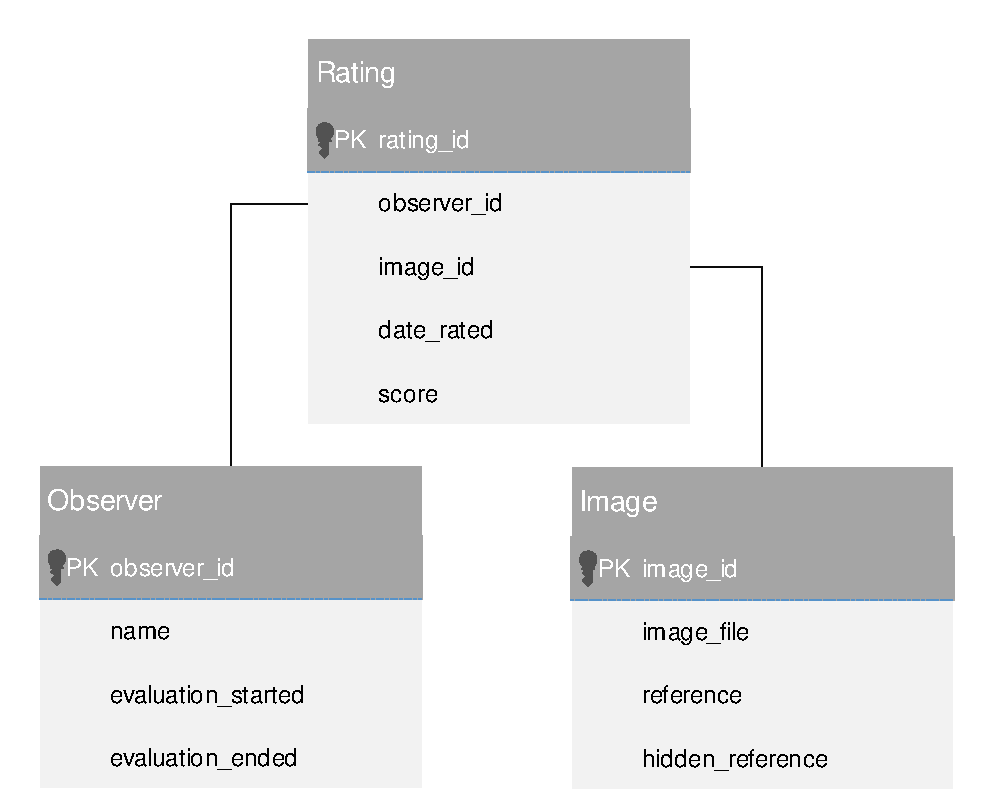
\includegraphics[width = 270pt]{Img/model.pdf}
	\caption{The architecture of the database.}
	\label{fig:database_architecture}
\end{figure}

The Observer table will contain information about all observers who have completed the quality evaluation. Each observer is created with a unique id, a name and the start and end time of the evaluation. The time stamps will be used to investigate the amount of time the observer has spent on the evaluation. This is relevant only if the evaluation is suspicious.

The Image table will contain information about all images in the evaluation. Each image is created with a unique id, a path to the image(image\_file), and the information of whether or not the image is being used as a reference or a hidden reference.

The Rating table will contain information about all ratings which have been made throughout all evaluations. Each rating will be created with a unique id, two foreign keys (observer\_id and image\_id) that refer to a primary key in the Observer and Image table respectively, the time of the rating and the score of the particular image.

% subsection model (end)

\subsection{Template} % (fold)
\label{sub:template}

The template is the front-end of the web application which typically consists of HTML/CSS. Django offers a powerful template engine that supports the developer in doing presentation logic. The design of the template is done with respect to descriptions of the SAMVIQ interface found in \cite{InternationalTelecommunicationUnion2007} and \cite{Street}. A mockup of the template is illustrated in \autoref{fig:template_mockup}.

\begin{figure}[H]
	\centering
	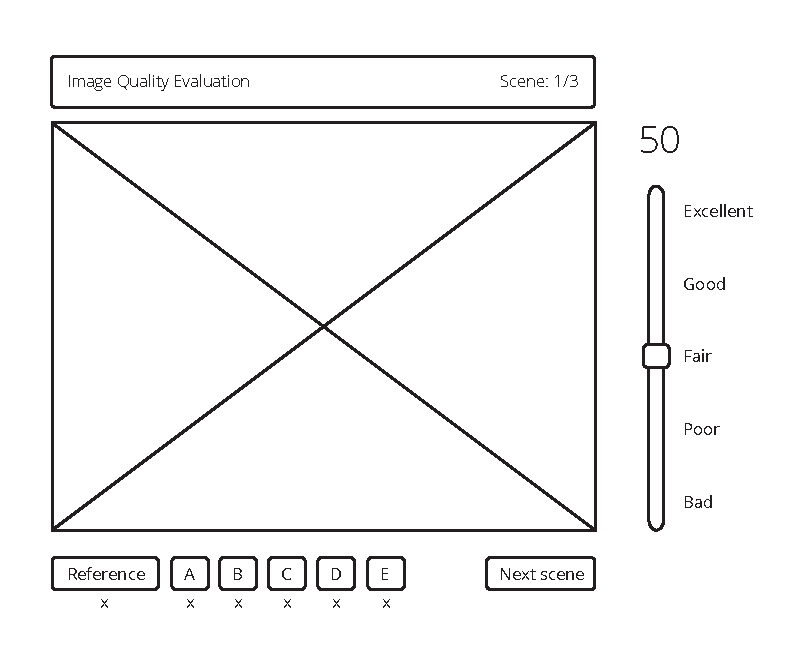
\includegraphics[width = 290pt]{Img/mockup.pdf}
	\caption{Mockup of the template.}
	\label{fig:template_mockup}
\end{figure}

According to both articles the template should consist of a large image in the middle. Below the image navigation buttons should be placed, one labeled as 'Reference' and the rest labeled alphabetically. A button for changing to the next scene should also be present. 

Both articles state that the rating mechanism as a slider located on the right side of the image. The slider has the five rating labels spread out over the total range. The score is shown both at the top of the slider and under the button which links to the image.

According to both articles the background color is chosen to be mid-range gray although this is not shown in the mockup. Above the image, information about the process is shown in order to let the observer be aware about the number of remaining scenes to evaluate.

% subsection template (end)

\subsection{View} % (fold)
\label{sub:view}

The view performs the requested action from the observer which typically involves reading from and writing to the database. This view instance is responsible for creating a new observer when a new evaluation is started. It also has to save all ratings done in a scene before changing to the next scene.

% subsection view (end)

% section the_web_application (end)